\section{Theoretical Analysis}
\label{sec:analysis}

\subsection{Envelope Detector Circuit Output}
\label{subsec:theo_edc}

In this subsection, we present the theoretical approach used for determining the output of the Envelope Detector Circuit, and the resulting plot.

Firstly, the $v_{in}$ voltage needs to have its amplitude reduced. To achieve that, a transformer with 1:17 ratio is used and the AC voltage dropping form node 1 to node 2 is given by equation \ref{eq:vtrans}.

\begin{equation}
    v_{trans}(t) = \frac{A_{in}}{n} \cdot cos(\omega \cdot t)
    \label{eq:vtrans}
\end{equation}


where $A_{in}$ is the amplitude of the original signal $v_{in}$, $n=17$, $\omega=2 \cdot pi \cdot f$, and $f=50Hz$.

Secondly, a envelope detector circuit is used, composed of a full-wave bridge rectifier circuit and a capacitor. The full-wave bridge rectifier consists of four diodes and a resistor, and the ideal diode model is used. 

As shown in theoretical classes, the output voltage of the envelope detector $v_3$ from $t=0$ to $t_{off}$ is equal to the absolute value of $v_{trans}$. The instant $t_{off}$ can be determined using equation \ref{eq:toff}.

\begin{equation}
t_{off} = \frac{arctan({\frac{1}{\cdot R \cdot C \cdot \omega})}}{\omega}
\label{eq:toff}
\end{equation}

From then on, $v_3$ is computed as equation \ref{eq:v3}

\begin{equation}
    v_3(t) = \frac{A_{in}}{n} \cdot cos({\omega \cdot t_{off}}) \cdot e^{\frac{t-t_{off}}{R_{1} \cdot C}}
    \label{eq:v3}
\end{equation}

until the absolute value of $v_{trans}$ is greater than equation \ref{eq:v3}. After that, $v_3$ equals again the absolute value of $v_{trans}$, until the next $t_{off}$, which comes half the wave period after the previous one, and so on. Note that, in $v_3$, the frequency has doubled.

\subsection{Voltage Regulator Circuit}
\label{subsec:theo_vr}

In this subsection, incremental analysis is used to compute the AC component of $v_4$ ($v_{4_{AC}}$) and, subsequently, $v_4(t)$ as a whole. Incremental analysis was used. In order to achieve the subsection's goal, we need to obtain $r_d$ (incremental diode resistance) and, as learned in theoretical classes, it is as follows

\begin{equation}
    r_d = \frac{\eta \cdot V_T}{I_S \cdot e^{\frac{V_{ON}}{\eta \cdot V_T}}}
    \label{eq:rd}
\end{equation}

in which $I_S=1e-14$, $V_T=0.025$, $\eta = 1$ and $V_{ON}=0.7$ (as an estimated approximation).

To obtain $v_{4_{AC}}$, equation \ref{eq:v4ac} is used,

\begin{equation}
    v_{4_{AC}}(t) = \frac{17 \cdot r_d}{17 \cdot r_d + R_2} \cdot v_3(t).
    \label{eq:v4ac}
\end{equation}

since there are 17 diodes in series.

Adding to the aforementioned signal its DC component, which is $V_{ON}$ multiplied by the number of diodes (17), $v_4(t)$ can be computed.

With this theoretical approach, the plots in Figure \ref{plot:todas} and Figure \ref{plot:diferenca} can be obtained. 


\begin{figure}[h]
\centering
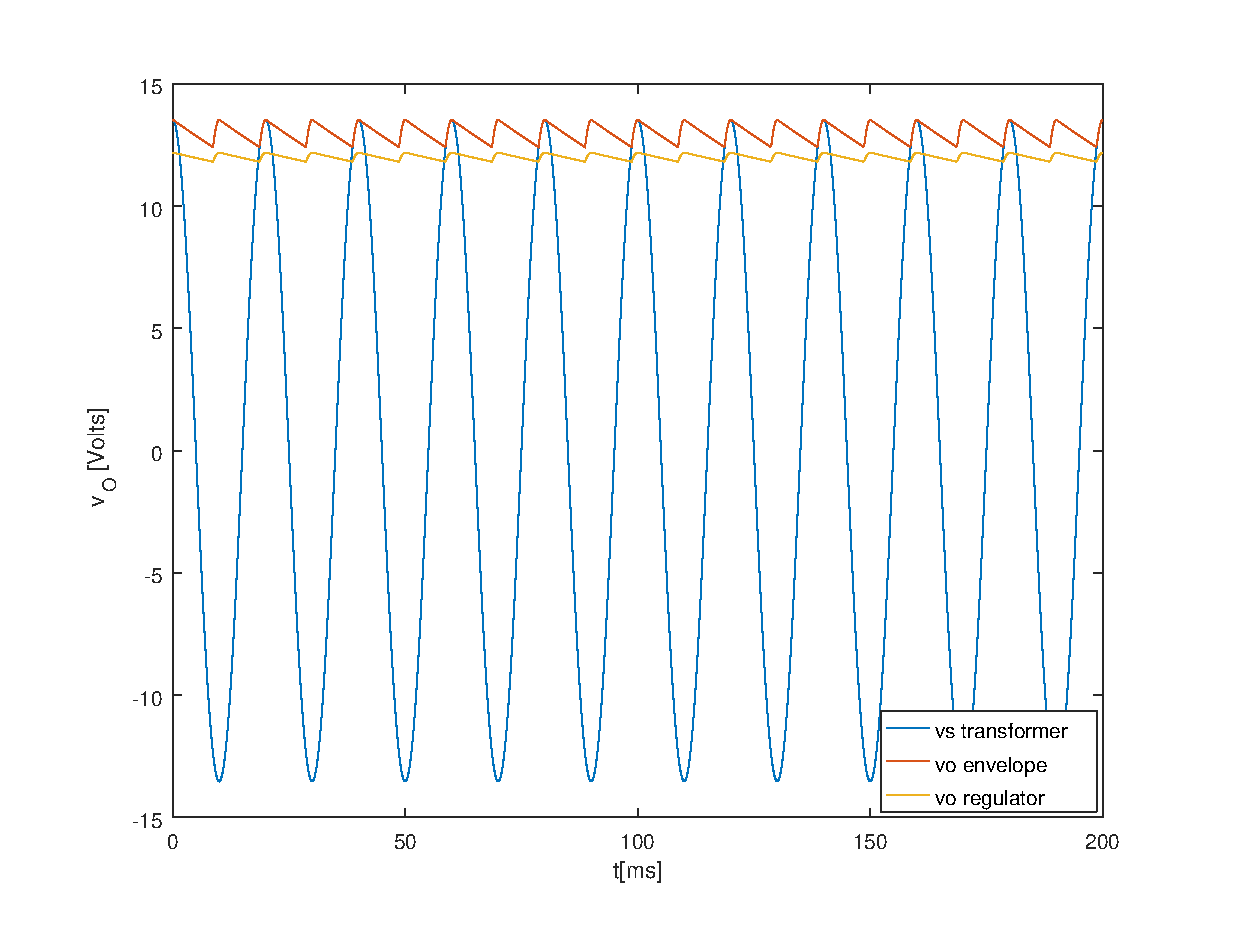
\includegraphics[width=0.6\linewidth]{V_todas.eps}
\caption{Voltages $v_{trans}(t)$ ("vs in transformer"), $v_3(t)$ ("v in envelope") and $v_4(t)$ ("v in regulator").}
\label{plot:todas}
\end{figure}

\begin{figure}[h]
\centering
\includegraphics[width=0.6\linewidth]{diferenca.eps}
\caption{Output voltage $v_4(t)$ minus 12 V.}
\label{plot:diferenca}
\end{figure}

\clearpage


Lastly, the voltage ripple is calculated through equation \ref{eq:vripple}.

\begin{equation}
    V_{Ripple} = max(v_4(t)) - min(v_4(t))
    \label{eq:vripple}
\end{equation}

and we are able to obtain 

\begin{equation}
    V_{Ripple} = 0.008643 V
\end{equation}
\begin{equation}
    DC Level = 11.9 V
\end{equation}

\subsection{Cost and Merit}
\label{subsec:theo_merit}

Using the cost information described in Section \ref{sec:introduction}, the cost of the circuit is

\begin{equation}
    cost = 33.74 MU
\end{equation}

Considering the Merit equation given, the Merit score is

\begin{equation}
    M = 0.2728
\end{equation}
